\scanpage{32}

\margin{\figure{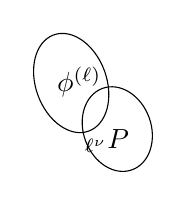
\begin{tikzpicture}\node (a) at (0,.3) {$\phi^{(\ell)}$};\node (b) at (.35,-.45) {${}_{\ell^\nu}P$};\draw[rotate=20] (0,.3) ellipse (.45 and .65);\draw[rotate=20] (.35,-.45) ellipse (.43 and .55);\end{tikzpicture}}}
\[
(2.2.4)\qquad\deleted{\unsure{\$}}\phi^{(\ell)}_\xi\deleted{\unsure{\$}}=(\phi^{\ell^\nu}_\xi)_{\nu\geq0},\quad\text{où}\quad\phi^{\ell^\nu}_\xi:{}_{\ell^\nu}P\times{}_{\ell^\nu}Q\longrightarrow G.
\]
Les diagrammes \deleted{déduits}\inserted{commutatifs} de (2.2.2) en y faisant $n=\ell^\nu$, $n'=\ell^{\nu'}$, pour $\nu'\geq\nu$, montrent que $\phi^{(\ell)}_\xi$ peut être interprété comme un accouplement de \deleted{\unsure{progroupes}} systèmes projectifs de groupes
\[
(2.2.5)\qquad\phi^{(\ell)}_\xi:T_\ell(P)\times T_\ell(Q)\longrightarrow T_\ell(G),
\]
où, pour un groupe $M$ de $T$ et un nombre premier $\ell$, on désigne par
\[
T_\ell(M)=({}_{\ell^\nu}M)_{\nu\geq0}
\]
le système projectif des ${}_{\ell^\nu}M$. L'accouplement \deleted{\unsure{\$}} (2.2.5) est encore appelé \uline{l'accouplement} $\ell$\uline{-adique associé à} $\xi$ (ou à la biextension $E$ de classe $\xi$). Pour $\xi$ variable, on obtient un homomorphisme canonique
\[
(2.2.6)\qquad\operatorname{Biext}^{\inserted{1}}(P,Q;G)\longrightarrow\operatorname{Hom}(T_\ell(P)\otimes T_\ell(Q),T_\ell(G)).
\]
On notera que les homomorphismes (2.1.2) sont \uline{fonctoriels} en $P,Q,G$ (pour $n$ fixé), d'où on déduit qu'il en est de même de (2.2.6).

\figure{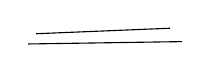
\begin{tikzpicture}\draw (0,0)--(1.7,.07);\draw (-.1,-.13)--(1.85,-.1);\end{tikzpicture}}

2.3. \deleted{On peut regarder} La compatibilité (2.2.2) permet de retrouver $\phi^n_\xi$ connaissant $\phi^{n'}_\xi$, pourvu que ${}_{n'}Q\xrightarrow{m}{}_nQ$ \inserted{soit} un épimorphisme, --- \deleted{\unsure{(NB la}} condition satisfaite, comme il est bien connu, si $nQ=Q$. En effet, comme ${}_{n'}P\xrightarrow{m}{}_nP$ est aussi un épimorphisme, $\phi^n_\xi$ se déduit alors de $\phi^{n'}_\xi$ par passage au quotient. On peut cependant \inserted{donner} une compatibilité légèrement plus précise que (2.2.2), qui permet d\deleted{\unsure{e}}'exprimer $\phi^n$ en termes de $\phi^{n'}$ sans aucune restriction sur $Q$, par la commutativité de

(2.3.1)
\diagram{\begin{tikzcd}[ampersand replacement=\&, column sep=small,row sep=large]
{}_{n'}P \arrow[d,"m"'] \& \times \& {}_nQ \arrow[d,"\mathrm{id}"] \arrow[rr,"{\phi^{n'}_\xi|_{{}_{n'}P\times{}_nQ}}"] \& \& {}_nG \arrow[d,"\mathrm{id}"]\\
{}_{\deleted{\unsure{m}}n}P \& \times \& {}_nQ \arrow[rr,"\phi^n_\xi"] \& \& {}_nG
\end{tikzcd}},

en formules
\[
(2.3.2)\qquad\phi^n_\xi(mx,y)=\phi^{n'}_\xi(x,y)\qquad(x\in{}_{n'}P(S),\ y\in{}_nQ(S)).
\]
Cette formule implique évidemment la commutativité de (2.2.2), qui s'écrit en effet
\[
\inserted{(2.3.3)}\qquad\phi^n_\xi(mx,my)=m\phi^{n'}_\xi(x,y)\qquad(x\in{}_{n'}P(S),\ y\in{}_{n'}P(S)),
\]
\margin{31}
